\documentclass[12pt,a4paper]{report}
\usepackage[utf8]{inputenc}				% Support de l'UTF-8			%
\usepackage[T1]{fontenc}				%
\usepackage{graphicx}					%
\usepackage[a4paper,					% Définit les marges
	headheight=45pt,headsep=35pt,		%
	left=1in,right=1in,					%
	top=1.6in,bottom=1.2in]{geometry}	%
\usepackage{lastpage} 					% Numérotation des pages
\usepackage{fancyhdr}					% Pour le header et le footer
\usepackage[normalem]{ulem}				% Soulignement
\usepackage{framed}						% Pour les tableaux des E/S
\usepackage{tcolorbox}			%
\usepackage{multicol}					% Gestion du nombre de colonnes
\usepackage{wrapfig}					%
\usepackage{caption}					% Centrage de la légende

% Justification du texte
\newcommand*\justify{		%
  \fontdimen2\font=0.4em	% interword space
  \fontdimen3\font=0.2em	% interword stretch
  \fontdimen4\font=0.1em	% interword shrink
  \fontdimen7\font=0.1em	% extra space
  \hyphenchar\font=`\-		% allowing hyphenation
}

% Infos du document
\author{INSAlgo}
\title{ShaKer 2019 PreCoding Battle - Problem A}

% En-tête et pied de page
\pagestyle{fancy}
\renewcommand{\headrulewidth}{0pt}				% Pas de bordure sous l'en-tête
\lhead{{\huge ShaKer 2019 PreCoding Battle}}		% En-tête gauche
\rhead{
\includegraphics[width=4cm]{logo.png}}	% En-tête droit
\rfoot{Page \thepage\,/\,\pageref{LastPage}}	% Pied de page droit
\cfoot{}										% Pied de page central

\begin{document}

\begin{center}
	{\Large A. "Bus Trip"}
	\bigskip
\end{center}

\section*{Statement}

\begin{wrapfigure}{r}{0.5\textwidth}
    \centering
    \captionsetup{justification=centering}
    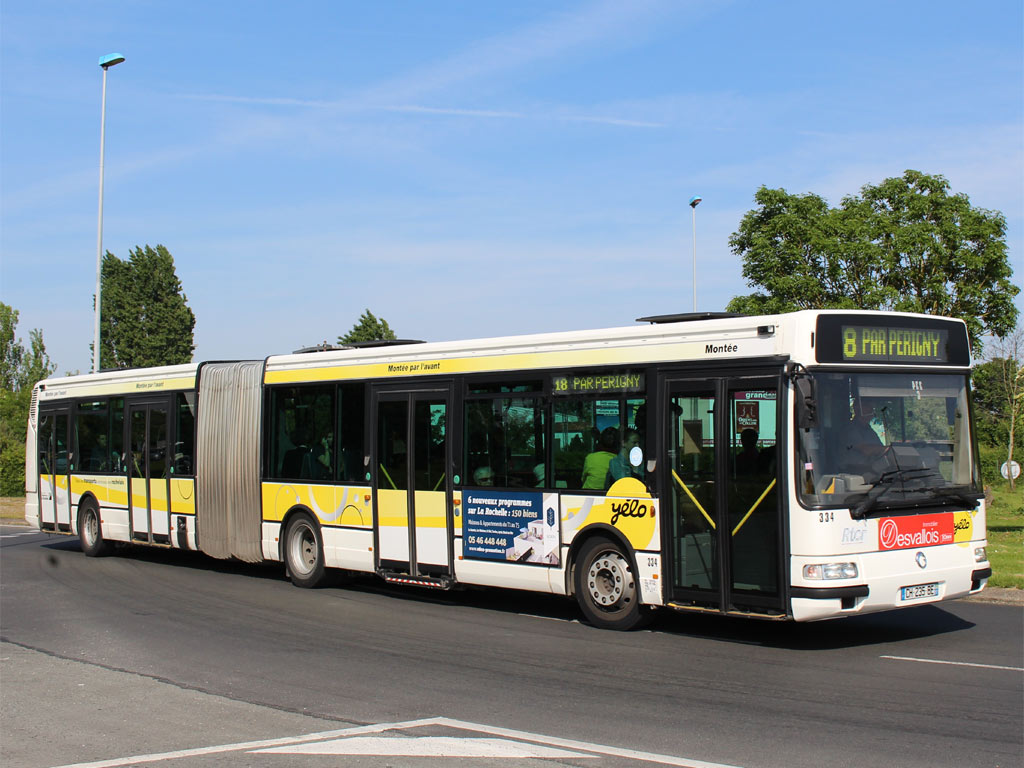
\includegraphics[width=0.45\textwidth]{bus.jpg}
    \caption*{A bus from your company}
\end{wrapfigure}
As the leader of a national bus transport company, you are facing a major technical issue : a retirement home wishes to organize a trip to a museum, without knowing how many buses will be needed.

You are thus going to write a program in order to solve this problem by computing the number of buses needed to carry every passenger to the museum.

\subsection*{Input}%Section des INPUT
On 2 lines~:
\begin{itemize}
\item An integer $N$ corresponding to the number of people who will need transportation to the museum ($0 \leq N \leq 10^{4}$)~;
\item An integer $P$ corresponding to the number of free seats on a bus ($1 \leq P \leq 10^{4}$).
\end{itemize}
\textit{NB~: All buses have the same capacity.}

\subsection*{Output}
\begin{itemize} %Section des OUTPUT
\item Print an integer (on the standard output) corresponding to the number of buses needed.
\end{itemize}

\section*{Example}%Section Exemple
\begin{minipage}{\linewidth}

%Pour un exemple copier d'ici à ...
\begin{multicols}{2}
	\begin{tcolorbox}[title=Input,width=\linewidth,arc=0mm,colbacktitle={white!80!black},coltitle=black]
		\begin{verbatim}
10
5
		\end{verbatim}
	\end{tcolorbox}
\columnbreak
	\begin{tcolorbox}[title=Output,width=\linewidth,arc=0mm,colbacktitle={white!80!black},coltitle=black]
		\begin{verbatim}
2
        \end{verbatim}
	\end{tcolorbox}
\end{multicols}
Here, 10 passengers need transportation and each bus has 5 free seats~; 2 buses are thus needed.
%... à ici pour la fin d'un exemple. Penser à mettre plusieurs exemples

%Pour un exemple copier d'ici à ...
\begin{multicols}{2}
	\begin{tcolorbox}[title=Input,width=\linewidth,arc=0mm,colbacktitle={white!80!black},coltitle=black]
		\begin{verbatim}
17
7
		\end{verbatim}
	\end{tcolorbox}
\columnbreak
	\begin{tcolorbox}[title=Output,width=\linewidth,arc=0mm,colbacktitle={white!80!black},coltitle=black]
		\begin{verbatim}
3
        \end{verbatim}
	\end{tcolorbox}
\end{multicols}
%... à ici pour la fin d'un exemple. Penser à mettre plusieurs exemples
In this case, 17 passengers need to be transported using 7-seat buses, we therefore need at least 3 buses (with 21 seats in total).
\end{minipage}

\bigskip



\end{document}